% Options for packages loaded elsewhere
\PassOptionsToPackage{unicode}{hyperref}
\PassOptionsToPackage{hyphens}{url}
\PassOptionsToPackage{dvipsnames,svgnames,x11names}{xcolor}
%
\documentclass[
  letterpaper,
  DIV=11,
  numbers=noendperiod]{scrartcl}
\usepackage{amsmath,amssymb}
\usepackage{lmodern}
\usepackage{iftex}
\ifPDFTeX
  \usepackage[T1]{fontenc}
  \usepackage[utf8]{inputenc}
  \usepackage{textcomp} % provide euro and other symbols
\else % if luatex or xetex
  \usepackage{unicode-math}
  \defaultfontfeatures{Scale=MatchLowercase}
  \defaultfontfeatures[\rmfamily]{Ligatures=TeX,Scale=1}
\fi
% Use upquote if available, for straight quotes in verbatim environments
\IfFileExists{upquote.sty}{\usepackage{upquote}}{}
\IfFileExists{microtype.sty}{% use microtype if available
  \usepackage[]{microtype}
  \UseMicrotypeSet[protrusion]{basicmath} % disable protrusion for tt fonts
}{}
\makeatletter
\@ifundefined{KOMAClassName}{% if non-KOMA class
  \IfFileExists{parskip.sty}{%
    \usepackage{parskip}
  }{% else
    \setlength{\parindent}{0pt}
    \setlength{\parskip}{6pt plus 2pt minus 1pt}}
}{% if KOMA class
  \KOMAoptions{parskip=half}}
\makeatother
\usepackage{xcolor}
\usepackage{color}
\usepackage{fancyvrb}
\newcommand{\VerbBar}{|}
\newcommand{\VERB}{\Verb[commandchars=\\\{\}]}
\DefineVerbatimEnvironment{Highlighting}{Verbatim}{commandchars=\\\{\}}
% Add ',fontsize=\small' for more characters per line
\usepackage{framed}
\definecolor{shadecolor}{RGB}{241,243,245}
\newenvironment{Shaded}{\begin{snugshade}}{\end{snugshade}}
\newcommand{\AlertTok}[1]{\textcolor[rgb]{0.68,0.00,0.00}{#1}}
\newcommand{\AnnotationTok}[1]{\textcolor[rgb]{0.37,0.37,0.37}{#1}}
\newcommand{\AttributeTok}[1]{\textcolor[rgb]{0.40,0.46,0.14}{#1}}
\newcommand{\BaseNTok}[1]{\textcolor[rgb]{0.68,0.00,0.00}{#1}}
\newcommand{\BuiltInTok}[1]{\textcolor[rgb]{0.00,0.46,0.62}{#1}}
\newcommand{\CharTok}[1]{\textcolor[rgb]{0.13,0.47,0.30}{#1}}
\newcommand{\CommentTok}[1]{\textcolor[rgb]{0.37,0.37,0.37}{#1}}
\newcommand{\CommentVarTok}[1]{\textcolor[rgb]{0.37,0.37,0.37}{\textit{#1}}}
\newcommand{\ConstantTok}[1]{\textcolor[rgb]{0.56,0.35,0.01}{#1}}
\newcommand{\ControlFlowTok}[1]{\textcolor[rgb]{0.00,0.46,0.62}{#1}}
\newcommand{\DataTypeTok}[1]{\textcolor[rgb]{0.68,0.00,0.00}{#1}}
\newcommand{\DecValTok}[1]{\textcolor[rgb]{0.68,0.00,0.00}{#1}}
\newcommand{\DocumentationTok}[1]{\textcolor[rgb]{0.37,0.37,0.37}{\textit{#1}}}
\newcommand{\ErrorTok}[1]{\textcolor[rgb]{0.68,0.00,0.00}{#1}}
\newcommand{\ExtensionTok}[1]{\textcolor[rgb]{0.00,0.46,0.62}{#1}}
\newcommand{\FloatTok}[1]{\textcolor[rgb]{0.68,0.00,0.00}{#1}}
\newcommand{\FunctionTok}[1]{\textcolor[rgb]{0.28,0.35,0.67}{#1}}
\newcommand{\ImportTok}[1]{\textcolor[rgb]{0.00,0.46,0.62}{#1}}
\newcommand{\InformationTok}[1]{\textcolor[rgb]{0.37,0.37,0.37}{#1}}
\newcommand{\KeywordTok}[1]{\textcolor[rgb]{0.00,0.46,0.62}{#1}}
\newcommand{\NormalTok}[1]{\textcolor[rgb]{0.00,0.46,0.62}{#1}}
\newcommand{\OperatorTok}[1]{\textcolor[rgb]{0.37,0.37,0.37}{#1}}
\newcommand{\OtherTok}[1]{\textcolor[rgb]{0.00,0.46,0.62}{#1}}
\newcommand{\PreprocessorTok}[1]{\textcolor[rgb]{0.68,0.00,0.00}{#1}}
\newcommand{\RegionMarkerTok}[1]{\textcolor[rgb]{0.00,0.46,0.62}{#1}}
\newcommand{\SpecialCharTok}[1]{\textcolor[rgb]{0.37,0.37,0.37}{#1}}
\newcommand{\SpecialStringTok}[1]{\textcolor[rgb]{0.13,0.47,0.30}{#1}}
\newcommand{\StringTok}[1]{\textcolor[rgb]{0.13,0.47,0.30}{#1}}
\newcommand{\VariableTok}[1]{\textcolor[rgb]{0.07,0.07,0.07}{#1}}
\newcommand{\VerbatimStringTok}[1]{\textcolor[rgb]{0.13,0.47,0.30}{#1}}
\newcommand{\WarningTok}[1]{\textcolor[rgb]{0.37,0.37,0.37}{\textit{#1}}}
\usepackage{longtable,booktabs,array}
\usepackage{calc} % for calculating minipage widths
% Correct order of tables after \paragraph or \subparagraph
\usepackage{etoolbox}
\makeatletter
\patchcmd\longtable{\par}{\if@noskipsec\mbox{}\fi\par}{}{}
\makeatother
% Allow footnotes in longtable head/foot
\IfFileExists{footnotehyper.sty}{\usepackage{footnotehyper}}{\usepackage{footnote}}
\makesavenoteenv{longtable}
\usepackage{graphicx}
\makeatletter
\def\maxwidth{\ifdim\Gin@nat@width>\linewidth\linewidth\else\Gin@nat@width\fi}
\def\maxheight{\ifdim\Gin@nat@height>\textheight\textheight\else\Gin@nat@height\fi}
\makeatother
% Scale images if necessary, so that they will not overflow the page
% margins by default, and it is still possible to overwrite the defaults
% using explicit options in \includegraphics[width, height, ...]{}
\setkeys{Gin}{width=\maxwidth,height=\maxheight,keepaspectratio}
% Set default figure placement to htbp
\makeatletter
\def\fps@figure{htbp}
\makeatother
\setlength{\emergencystretch}{3em} % prevent overfull lines
\providecommand{\tightlist}{%
  \setlength{\itemsep}{0pt}\setlength{\parskip}{0pt}}
\setcounter{secnumdepth}{-\maxdimen} % remove section numbering
% Make \paragraph and \subparagraph free-standing
\ifx\paragraph\undefined\else
  \let\oldparagraph\paragraph
  \renewcommand{\paragraph}[1]{\oldparagraph{#1}\mbox{}}
\fi
\ifx\subparagraph\undefined\else
  \let\oldsubparagraph\subparagraph
  \renewcommand{\subparagraph}[1]{\oldsubparagraph{#1}\mbox{}}
\fi
\KOMAoption{captions}{tableheading}
\makeatletter
\makeatother
\makeatletter
\@ifpackageloaded{caption}{}{\usepackage{caption}}
\AtBeginDocument{%
\renewcommand*\contentsname{Table of contents}
\renewcommand*\listfigurename{List of Figures}
\renewcommand*\listtablename{List of Tables}
\renewcommand*\figurename{Figure}
\renewcommand*\tablename{Table}
}
\@ifpackageloaded{float}{}{\usepackage{float}}
\floatstyle{ruled}
\@ifundefined{c@chapter}{\newfloat{codelisting}{h}{lop}}{\newfloat{codelisting}{h}{lop}[chapter]}
\floatname{codelisting}{Listing}
\newcommand*\listoflistings{\listof{codelisting}{List of Listings}}
\makeatother
\makeatletter
\@ifpackageloaded{caption}{}{\usepackage{caption}}
\@ifpackageloaded{subcaption}{}{\usepackage{subcaption}}
\makeatother
\makeatletter
\@ifpackageloaded{tcolorbox}{}{\usepackage[many]{tcolorbox}}
\makeatother
\makeatletter
\@ifundefined{shadecolor}{\definecolor{shadecolor}{rgb}{.97, .97, .97}}
\makeatother
\makeatletter
\makeatother
\ifLuaTeX
  \usepackage{selnolig}  % disable illegal ligatures
\fi
\IfFileExists{bookmark.sty}{\usepackage{bookmark}}{\usepackage{hyperref}}
\IfFileExists{xurl.sty}{\usepackage{xurl}}{} % add URL line breaks if available
\urlstyle{same} % disable monospaced font for URLs
\hypersetup{
  pdftitle={Effectiveness of Contraception Methods},
  pdfauthor={Travis Dawry},
  colorlinks=true,
  linkcolor={blue},
  filecolor={Maroon},
  citecolor={Blue},
  urlcolor={Blue},
  pdfcreator={LaTeX via pandoc}}

\title{Effectiveness of Contraception Methods}
\author{Travis Dawry}
\date{May 8, 2022}

\begin{document}
\maketitle

\ifdefined\Shaded\renewenvironment{Shaded}{\begin{tcolorbox}[sharp corners, frame hidden, enhanced, breakable, borderline west={3pt}{0pt}{shadecolor}, boxrule=0pt, interior hidden]}{\end{tcolorbox}}\fi

\hypertarget{purpose}{%
\subsection{Purpose}\label{purpose}}

Visualization to show the expected failure of typical contraception
methods.

Percentage of women experiencing an unintended pregnancy during the
first year of typical use.

Probability of at least one failure over N years, with typical use.

\hypertarget{source}{%
\subsection{Source}\label{source}}

Source of data is \emph{Contraceptive failure in the United States}.
Trussell,J. Contraception,2011,Vol.83(5),p.398

\hypertarget{code}{%
\subsection{Code}\label{code}}

\begin{Shaded}
\begin{Highlighting}[]
\FunctionTok{library}\NormalTok{(forcats)}
\FunctionTok{library}\NormalTok{(ggplot2)}
\FunctionTok{library}\NormalTok{(viridis)}
\end{Highlighting}
\end{Shaded}

\begin{verbatim}
Loading required package: viridisLite
\end{verbatim}

\begin{Shaded}
\begin{Highlighting}[]
\FunctionTok{library}\NormalTok{(tibble)}
\FunctionTok{library}\NormalTok{(tidyr)}
\end{Highlighting}
\end{Shaded}

\begin{Shaded}
\begin{Highlighting}[]
\NormalTok{none }\OtherTok{\textless{}{-}} \FloatTok{0.85}
\NormalTok{withdrawal }\OtherTok{\textless{}{-}} \FloatTok{0.22}
\NormalTok{condom }\OtherTok{\textless{}{-}} \FloatTok{0.18}
\NormalTok{pill }\OtherTok{\textless{}{-}} \FloatTok{0.09}
\NormalTok{IUD }\OtherTok{\textless{}{-}} \FloatTok{0.008}
\NormalTok{iud\_progestin }\OtherTok{\textless{}{-}} \FloatTok{0.002}
\NormalTok{female\_ster }\OtherTok{\textless{}{-}} \FloatTok{0.005}
\NormalTok{male\_ster }\OtherTok{\textless{}{-}} \FloatTok{0.0015}
\end{Highlighting}
\end{Shaded}

\begin{Shaded}
\begin{Highlighting}[]
\NormalTok{FailRate }\OtherTok{\textless{}{-}} \ControlFlowTok{function}\NormalTok{(years, method)\{}
     \FunctionTok{pbinom}\NormalTok{(}\DecValTok{0}\NormalTok{, years, method, }\AttributeTok{lower.tail =} \ConstantTok{FALSE}\NormalTok{)}
\NormalTok{\}}

\NormalTok{PlotFailRate }\OtherTok{\textless{}{-}} \ControlFlowTok{function}\NormalTok{(years, method)\{}
\NormalTok{     rate }\OtherTok{\textless{}\textless{}{-}} \FunctionTok{pbinom}\NormalTok{(}\DecValTok{0}\NormalTok{, }\DecValTok{1}\SpecialCharTok{:}\NormalTok{years, method, }\AttributeTok{lower.tail =} \ConstantTok{FALSE}\NormalTok{)}
\NormalTok{     p }\OtherTok{\textless{}{-}} \FunctionTok{ggplot}\NormalTok{(}\FunctionTok{as.data.frame}\NormalTok{(rate), }\FunctionTok{aes}\NormalTok{(}\AttributeTok{x =} \FunctionTok{seq}\NormalTok{(}\DecValTok{1}\SpecialCharTok{:}\FunctionTok{length}\NormalTok{(rate)), }\AttributeTok{y =}\NormalTok{ rate))}

\NormalTok{     p }\SpecialCharTok{+}
     \FunctionTok{geom\_line}\NormalTok{(}\FunctionTok{aes}\NormalTok{(}\AttributeTok{color =}\NormalTok{ rate)) }\SpecialCharTok{+}
     \FunctionTok{scale\_colour\_gradient}\NormalTok{(}\AttributeTok{high =} \StringTok{"red"}\NormalTok{)}
\NormalTok{\}}
\end{Highlighting}
\end{Shaded}

\begin{Shaded}
\begin{Highlighting}[]
\FunctionTok{FailRate}\NormalTok{(}\DecValTok{4}\NormalTok{, condom)}
\end{Highlighting}
\end{Shaded}

\begin{verbatim}
[1] 0.5478782
\end{verbatim}

\begin{Shaded}
\begin{Highlighting}[]
\FunctionTok{FailRate}\NormalTok{(}\DecValTok{4}\NormalTok{, condom }\SpecialCharTok{*}\NormalTok{ pill)}
\end{Highlighting}
\end{Shaded}

\begin{verbatim}
[1] 0.0632423
\end{verbatim}

\begin{Shaded}
\begin{Highlighting}[]
\FunctionTok{PlotFailRate}\NormalTok{(}\DecValTok{4}\NormalTok{, condom)}
\end{Highlighting}
\end{Shaded}

\begin{figure}[H]

{\centering 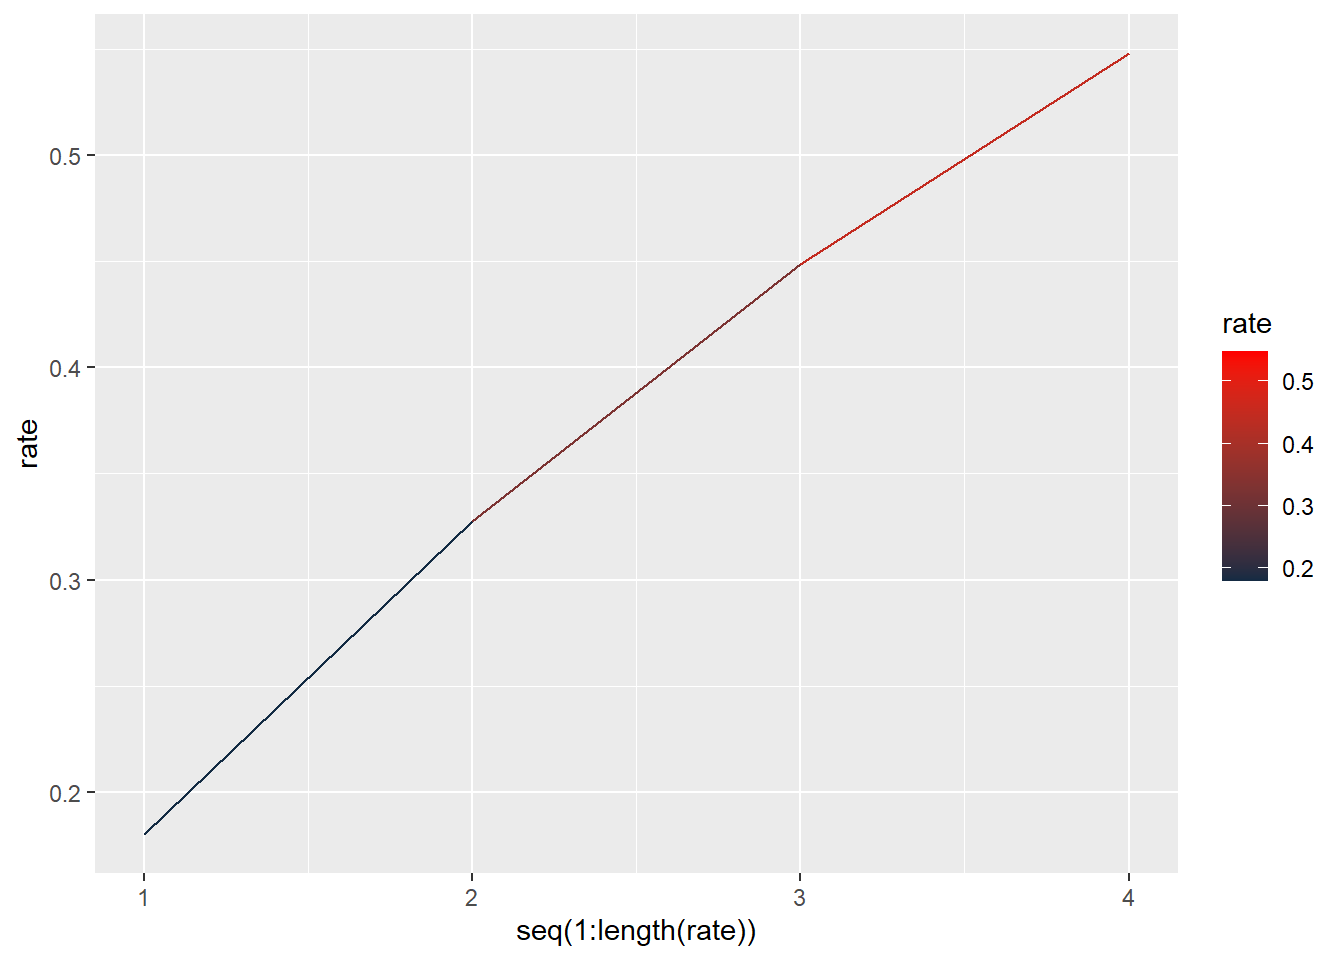
\includegraphics{eff_contraception_methods_files/figure-pdf/examples-1.pdf}

}

\end{figure}

\begin{Shaded}
\begin{Highlighting}[]
\FunctionTok{PlotFailRate}\NormalTok{(}\DecValTok{4}\NormalTok{, condom }\SpecialCharTok{*}\NormalTok{ pill)}
\end{Highlighting}
\end{Shaded}

\begin{figure}[H]

{\centering 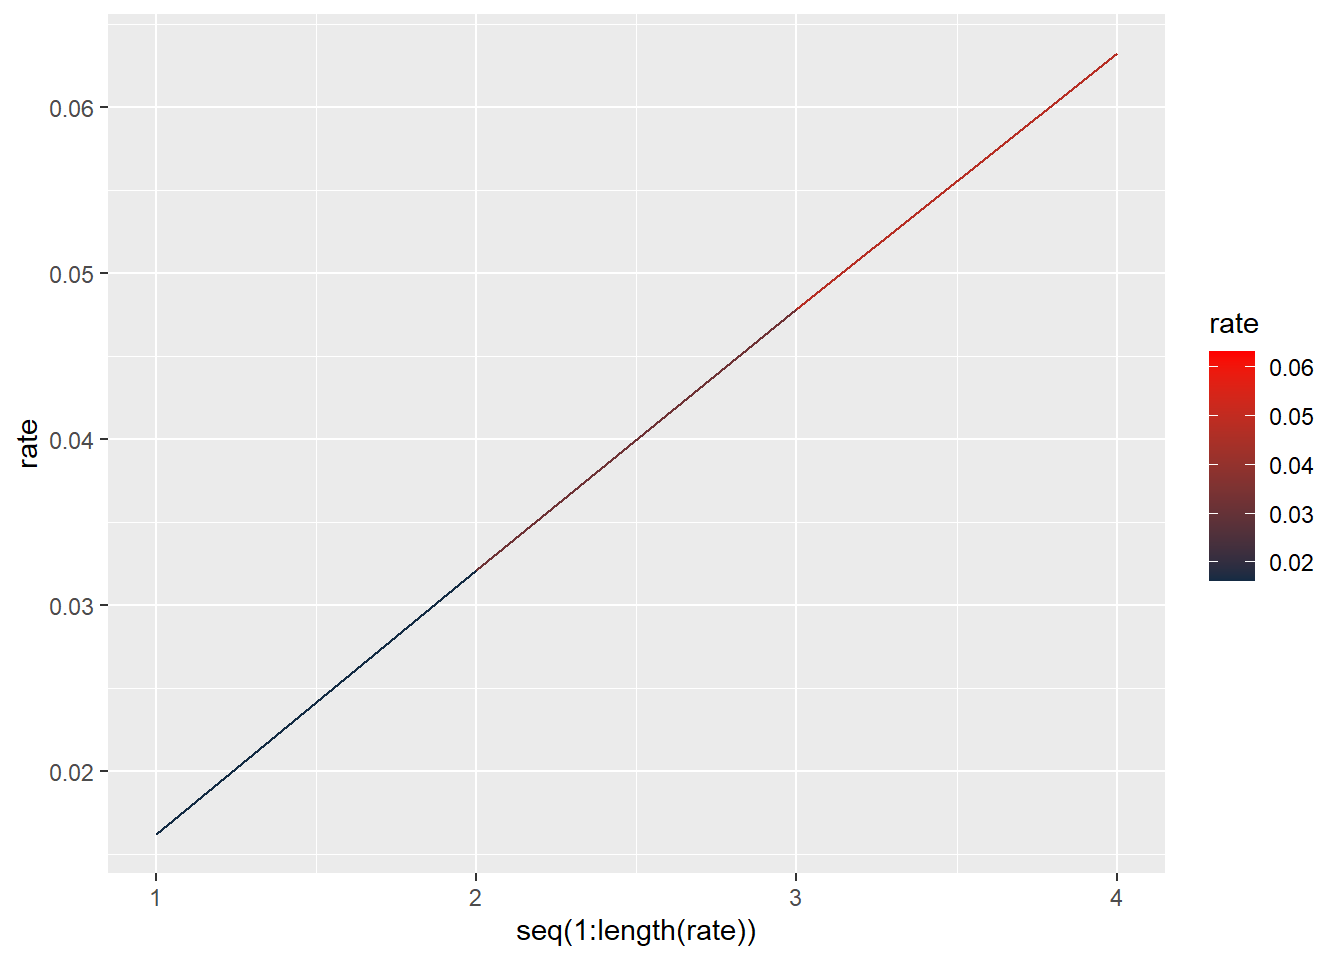
\includegraphics{eff_contraception_methods_files/figure-pdf/examples-2.pdf}

}

\end{figure}

\begin{Shaded}
\begin{Highlighting}[]
\NormalTok{lifetime\_failure }\OtherTok{\textless{}{-}} \FunctionTok{tibble}\NormalTok{(}\AttributeTok{years =} \DecValTok{1}\SpecialCharTok{:}\DecValTok{20}\NormalTok{,}
                           \AttributeTok{none =} \FunctionTok{FailRate}\NormalTok{(years, none),}
                           \AttributeTok{withdrawal =} \FunctionTok{FailRate}\NormalTok{(years, withdrawal),}
                           \AttributeTok{condom =} \FunctionTok{FailRate}\NormalTok{(years, condom),}
                           \AttributeTok{pill =} \FunctionTok{FailRate}\NormalTok{(years, pill),}
                           \AttributeTok{IUD =} \FunctionTok{FailRate}\NormalTok{(years, IUD))}

\NormalTok{failure\_table }\OtherTok{\textless{}{-}} \FunctionTok{pivot\_longer}\NormalTok{(lifetime\_failure, }\AttributeTok{cols =} \SpecialCharTok{{-}}\FunctionTok{c}\NormalTok{(years), }\AttributeTok{names\_to =} \StringTok{"method"}\NormalTok{, }\AttributeTok{values\_to =} \StringTok{"failure"}\NormalTok{)}

\NormalTok{failure\_table}\SpecialCharTok{$}\NormalTok{method }\OtherTok{\textless{}{-}} \FunctionTok{as.factor}\NormalTok{(failure\_table}\SpecialCharTok{$}\NormalTok{method)}

\NormalTok{failure\_table}\SpecialCharTok{$}\NormalTok{method }\OtherTok{\textless{}{-}} \FunctionTok{fct\_reorder}\NormalTok{(failure\_table}\SpecialCharTok{$}\NormalTok{method, failure\_table}\SpecialCharTok{$}\NormalTok{failure, }\AttributeTok{.fun =}\NormalTok{ mean, }\AttributeTok{.desc =} \ConstantTok{TRUE}\NormalTok{)}
\end{Highlighting}
\end{Shaded}

\begin{Shaded}
\begin{Highlighting}[]
\NormalTok{failure\_plot }\OtherTok{\textless{}{-}} \FunctionTok{ggplot}\NormalTok{(failure\_table) }\SpecialCharTok{+}
    \FunctionTok{aes}\NormalTok{(}\AttributeTok{x =}\NormalTok{ years, }\AttributeTok{y =}\NormalTok{ failure }\SpecialCharTok{*} \DecValTok{100}\NormalTok{, }\AttributeTok{colour =}\NormalTok{ method) }\SpecialCharTok{+}
    \FunctionTok{geom\_smooth}\NormalTok{(}\AttributeTok{size =} \DecValTok{1}\NormalTok{, }\AttributeTok{se =} \ConstantTok{FALSE}\NormalTok{, }\AttributeTok{method =} \StringTok{"loess"}\NormalTok{, }\AttributeTok{formula =} \StringTok{"y \textasciitilde{} x"}\NormalTok{) }\SpecialCharTok{+}
    \FunctionTok{geom\_hline}\NormalTok{(}\AttributeTok{yintercept =} \DecValTok{0}\NormalTok{) }\SpecialCharTok{+}
    \FunctionTok{scale\_colour\_viridis\_d}\NormalTok{(}\AttributeTok{option =} \StringTok{"D"}\NormalTok{, }\AttributeTok{direction =} \DecValTok{1}\NormalTok{) }\SpecialCharTok{+}
    \FunctionTok{scale\_x\_continuous}\NormalTok{(}\AttributeTok{expand =} \FunctionTok{expansion}\NormalTok{(}\DecValTok{0}\NormalTok{)) }\SpecialCharTok{+} 
    \FunctionTok{scale\_y\_continuous}\NormalTok{(}\AttributeTok{expand =} \FunctionTok{expansion}\NormalTok{(}\DecValTok{0}\NormalTok{)) }\SpecialCharTok{+}
    \FunctionTok{geom\_hline}\NormalTok{(}\AttributeTok{yintercept =} \DecValTok{25}\NormalTok{, }\AttributeTok{alpha =} \FloatTok{0.25}\NormalTok{) }\SpecialCharTok{+}
    \FunctionTok{geom\_hline}\NormalTok{(}\AttributeTok{yintercept =} \DecValTok{50}\NormalTok{, }\AttributeTok{alpha =} \FloatTok{0.25}\NormalTok{) }\SpecialCharTok{+}
    \FunctionTok{geom\_hline}\NormalTok{(}\AttributeTok{yintercept =} \DecValTok{75}\NormalTok{, }\AttributeTok{alpha =} \FloatTok{0.25}\NormalTok{) }\SpecialCharTok{+}
    \FunctionTok{ggtitle}\NormalTok{(}\StringTok{"Probability of At Least One Contraceptive Failure by Method"}\NormalTok{, }\AttributeTok{subtitle =} \StringTok{"With Typical Use"}\NormalTok{) }\SpecialCharTok{+}
    \FunctionTok{xlab}\NormalTok{(}\StringTok{"Years of Use"}\NormalTok{) }\SpecialCharTok{+}
    \FunctionTok{ylab}\NormalTok{(}\StringTok{"\% Chance of at Least One Pregnancy"}\NormalTok{) }\SpecialCharTok{+}
    \FunctionTok{theme\_bw}\NormalTok{()}

\NormalTok{failure\_plot}
\end{Highlighting}
\end{Shaded}

\begin{figure}[H]

{\centering 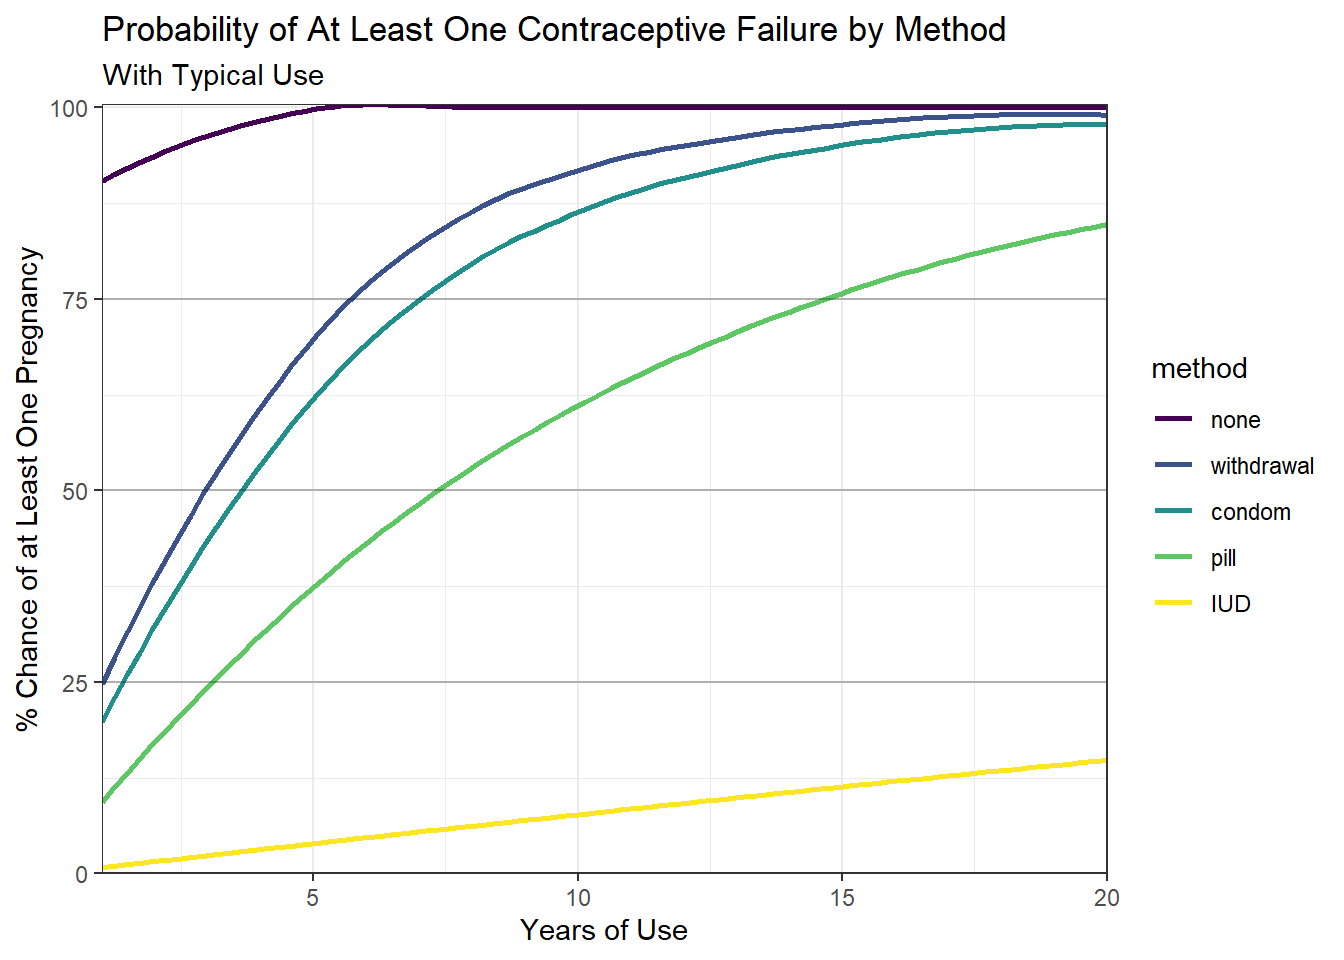
\includegraphics{eff_contraception_methods_files/figure-pdf/plot-1.pdf}

}

\end{figure}

\begin{Shaded}
\begin{Highlighting}[]
\NormalTok{ragg}\SpecialCharTok{::}\FunctionTok{agg\_png}\NormalTok{(}\StringTok{"failure\_plot\_16x9.png"}\NormalTok{, }\AttributeTok{width =} \DecValTok{16}\NormalTok{, }\AttributeTok{height =} \DecValTok{9}\NormalTok{, }\AttributeTok{units =} \StringTok{"in"}\NormalTok{, }\AttributeTok{res =} \DecValTok{300}\NormalTok{, }\AttributeTok{scaling =} \FloatTok{2.8}\NormalTok{)}
\NormalTok{failure\_plot}
\FunctionTok{dev.off}\NormalTok{()}
\end{Highlighting}
\end{Shaded}

\begin{verbatim}
pdf 
  2 
\end{verbatim}

\hypertarget{quarto}{%
\subsection{Quarto}\label{quarto}}

When you click the \textbf{Render} button a document will be generated
that includes both content and the output of embedded code. You can
embed code like this:

\begin{Shaded}
\begin{Highlighting}[]
\DecValTok{1} \SpecialCharTok{+} \DecValTok{1}
\end{Highlighting}
\end{Shaded}

\begin{verbatim}
[1] 2
\end{verbatim}

You can add options to executable code like this

\begin{verbatim}
[1] 4
\end{verbatim}

The \texttt{echo:\ false} option disables the printing of code (only
output is displayed).

\end{document}
